\documentclass[conference]{IEEEtran}
\IEEEoverridecommandlockouts

% ===== Packages =====
\usepackage[utf8]{inputenc}
\usepackage[T1]{fontenc}
\usepackage{cite}
\usepackage{amsmath,amssymb,amsfonts}
\usepackage{algorithmic}
\usepackage{graphicx}
\usepackage{textcomp}
\usepackage{xcolor}
\usepackage{booktabs}
\usepackage{multirow}
\usepackage{array}
\usepackage{url}
\usepackage{hyperref}
\usepackage{balance}
\usepackage{tikz}
\usetikzlibrary{arrows.meta,positioning,fit,shapes.geometric}

\def\BibTeX{{\rm B\kern-.05em{\sc i\kern-.025em b}\kern-.08em
    T\kern-.1667em\lower.7ex\hbox{E}\kern-.125emX}}

\begin{document}

\title{Abstractive Text Summarization Using a Transformer Implemented from Scratch and a Fine-tuned Pre-trained Language Model}

\author{
\IEEEauthorblockN{Mai Kha Anh, Nguyen Ngoc Dinh, Nguyen Thac Cuong, Nguyen Phi Anh}
\IEEEauthorblockA{\textit{Faculty of Information Technology} \\
\textit{University of Engineering and Technology, VNU}\\
Hanoi, Vietnam \\
Email: \{23020006, 23020009, 23030018, 23020021\}@vnu.edu.vn}
}

\maketitle

\begin{abstract}
Abstractive text summarization aims to generate a concise summary that preserves the main information of a long input document. In this project, we investigate two approaches for Vietnamese abstractive summarization. The first approach is a sequence-to-sequence Transformer implemented from scratch in PyTorch, including sinusoidal positional encoding, multi-head attention, encoder and decoder stacks, masking, training, and decoding utilities. The second approach, which uses a pre-trained language model with fewer than 3 billion parameters, is reserved for the next stage of the project. The implemented scratch Transformer has 11.47M trainable parameters and is evaluated using ROUGE-1, ROUGE-2, ROUGE-L, and repetition statistics. On the public test set, the Transformer with beam search obtains ROUGE-1 of 0.5747, ROUGE-2 of 0.2038, and ROUGE-L of 0.3045.
\end{abstract}

\begin{IEEEkeywords}
abstractive summarization, Transformer, sequence-to-sequence learning, pre-trained language model, ROUGE, Vietnamese NLP
\end{IEEEkeywords}

% =========================================================
\section{Introduction}
Text summarization is an important task in natural language processing (NLP), where the goal is to condense a long document into a shorter version while preserving the most important information. Summarization systems are useful in news aggregation, document search, information retrieval, education, and digital assistants. Compared with extractive summarization, which selects important sentences directly from the source document, abstractive summarization generates new sentences and can produce more natural and concise summaries.

In this project, we focus on abstractive text summarization. Given an input document $X = (x_1, x_2, \ldots, x_m)$, the system is required to generate a shorter target summary $Y = (y_1, y_2, \ldots, y_n)$, where $n < m$ in most cases. The generated summary should be fluent, concise, and faithful to the original content.

The project requires two parallel approaches. The first approach is to build and train a Transformer model from scratch. This means that the core components, including multi-head attention, positional encoding, encoder, decoder, and feed-forward network, must be implemented manually using basic PyTorch modules, without directly using high-level modules such as \texttt{nn.Transformer}. The second approach is to fine-tune a pre-trained language model with fewer than 3 billion parameters.

The main contributions of our work are as follows:
\begin{itemize}
    \item We implement a complete encoder-decoder Transformer architecture from scratch for abstractive summarization.
    \item We build the full data pipeline, including text cleaning, JSONL conversion, subword tokenizer training, tokenization cache creation, and mini-batch masking.
    \item We implement practical training and decoding improvements such as Pre-LN blocks, label smoothing, shared embeddings, weight tying, warmup scheduling, gradient clipping, beam search, length penalty, and no-repeat n-gram blocking.
    \item We evaluate the trained Transformer using ROUGE metrics, repetition statistics, validation decoding comparison, and the public test set.
\end{itemize}

% =========================================================
\section{Related Work}
Early neural summarization systems were commonly based on recurrent neural networks and sequence-to-sequence architectures with attention mechanisms. These models encode the input sequence into hidden representations and decode the summary token by token. However, recurrent models are difficult to parallelize and may struggle with long-range dependencies.

The Transformer architecture introduced by Vaswani et al. replaced recurrence with self-attention, allowing the model to capture dependencies between arbitrary positions in a sequence more efficiently. The original Transformer consists of an encoder stack and a decoder stack, where each layer contains attention mechanisms, feed-forward networks, residual connections, and layer normalization. Our implementation keeps this encoder-decoder structure and implements the core components manually, while using a few explicit training-oriented modifications described in the methodology.

Pre-trained language models further improved many NLP tasks by learning general-purpose representations from large-scale corpora. Models such as BART, T5, mBART, and PEGASUS are widely used for summarization because they are pre-trained with denoising or sequence-to-sequence objectives. Fine-tuning these models on a downstream summarization dataset often provides stronger results than training a model from scratch, especially when the task dataset is limited.

% =========================================================
\section{Methodology}

\subsection{Task Formulation}
The task is formulated as conditional sequence generation. Given a source document $X$, the model estimates the probability of a target summary $Y$ as:
\begin{equation}
P(Y|X) = \prod_{t=1}^{n} P(y_t | y_{<t}, X).
\end{equation}
During training, teacher forcing is used, where the decoder receives the previous ground-truth tokens. During inference, the summary is generated autoregressively until the end-of-sequence token is produced or the maximum decoding length is reached.

\subsection{Tokenization and Data Processing}
We use a SentencePiece BPE subword tokenizer trained on the provided training corpus. The preprocessing pipeline first inspects the parquet files, normalizes each example into a source--target pair, removes invalid or extremely short samples, and stores the cleaned data as JSONL files. The tokenizer then converts input documents and target summaries into sequences of token IDs. Special tokens include \texttt{<PAD>}, \texttt{<UNK>}, \texttt{<BOS>}, and \texttt{<EOS>}. Long documents are truncated to a maximum source length, and summaries are truncated to a maximum target length. Tokenized examples are cached as pickle files to avoid repeating the preprocessing step during training.

\begin{itemize}
    \item Tokenizer type: SentencePiece BPE
    \item Vocabulary size: 16000
    \item Maximum source length: 512 tokens
    \item Maximum target length: 128 tokens
    \item Filtering rules: source length from 30 to 900 words, target length from 3 to 180 words, and target/source length ratio at most 0.9
    \item Training samples: 10775
    \item Validation samples: 1349
    \item Test samples: 1344
\end{itemize}

\subsection{Transformer from Scratch}
Our first model is an encoder-decoder Transformer implemented from scratch. The model follows the main encoder-decoder design of the Transformer in \cite{vaswani2017attention}: token embeddings, sinusoidal positional encoding, multi-head attention, feed-forward networks, residual connections, encoder and decoder stacks, and a final vocabulary projection. For training stability and summarization quality, the implemented model intentionally uses Pre-LN blocks, GELU activation, shared source-target embeddings, output weight tying, label smoothing, warmup scheduling, beam search, length penalty, and no-repeat n-gram blocking. These changes are reported as implementation improvements rather than as exact components of the original paper.

\begin{figure*}[htbp]
\centering
\resizebox{0.95\textwidth}{!}{%
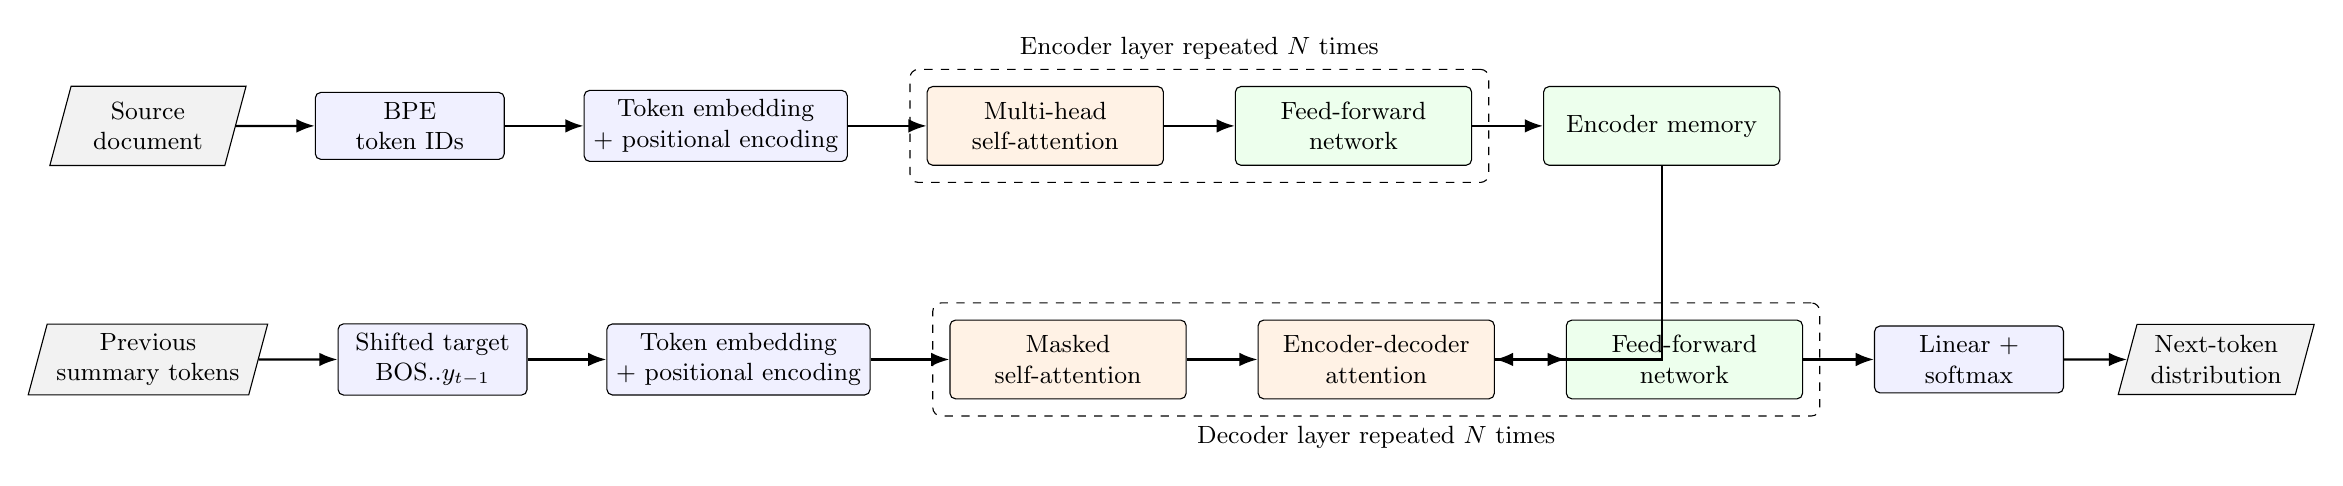
\begin{tikzpicture}[
    font=\small,
    box/.style={draw, rounded corners=2pt, align=center, minimum width=2.4cm, minimum height=0.85cm, fill=blue!6},
    block/.style={draw, rounded corners=2pt, align=center, minimum width=3.0cm, minimum height=1.0cm, fill=green!7},
    attn/.style={draw, rounded corners=2pt, align=center, minimum width=3.0cm, minimum height=1.0cm, fill=orange!10},
    io/.style={draw, trapezium, trapezium left angle=75, trapezium right angle=105, align=center, minimum width=2.5cm, minimum height=0.8cm, fill=gray!10},
    arrow/.style={-Latex, thick}
]
\node[io] (src) {Source\\document};
\node[box, right=1.0cm of src] (src_tok) {BPE\\token IDs};
\node[box, right=1.0cm of src_tok] (src_emb) {Token embedding\\+ positional encoding};
\node[attn, right=1.0cm of src_emb] (enc_attn) {Multi-head\\self-attention};
\node[block, right=0.9cm of enc_attn] (enc_ffn) {Feed-forward\\network};
\node[block, right=0.9cm of enc_ffn] (memory) {Encoder memory};

\node[io, below=2.0cm of src] (tgt) {Previous\\summary tokens};
\node[box, right=1.0cm of tgt] (tgt_tok) {Shifted target\\BOS..$y_{t-1}$};
\node[box, right=1.0cm of tgt_tok] (tgt_emb) {Token embedding\\+ positional encoding};
\node[attn, right=1.0cm of tgt_emb] (dec_self) {Masked\\self-attention};
\node[attn, right=0.9cm of dec_self] (cross) {Encoder-decoder\\attention};
\node[block, right=0.9cm of cross] (dec_ffn) {Feed-forward\\network};
\node[box, right=0.9cm of dec_ffn] (softmax) {Linear +\\softmax};
\node[io, right=0.8cm of softmax] (out) {Next-token\\distribution};

\draw[arrow] (src) -- (src_tok);
\draw[arrow] (src_tok) -- (src_emb);
\draw[arrow] (src_emb) -- (enc_attn);
\draw[arrow] (enc_attn) -- (enc_ffn);
\draw[arrow] (enc_ffn) -- (memory);
\draw[arrow] (tgt) -- (tgt_tok);
\draw[arrow] (tgt_tok) -- (tgt_emb);
\draw[arrow] (tgt_emb) -- (dec_self);
\draw[arrow] (dec_self) -- (cross);
\draw[arrow] (cross) -- (dec_ffn);
\draw[arrow] (dec_ffn) -- (softmax);
\draw[arrow] (softmax) -- (out);
\draw[arrow] (memory) |- (cross);

\node[draw, dashed, rounded corners=3pt, fit=(enc_attn)(enc_ffn), inner sep=6pt, label=above:{Encoder layer repeated $N$ times}] {};
\node[draw, dashed, rounded corners=3pt, fit=(dec_self)(cross)(dec_ffn), inner sep=6pt, label=below:{Decoder layer repeated $N$ times}] {};
\end{tikzpicture}
}
\caption{Architecture of the from-scratch encoder-decoder Transformer used for abstractive summarization. Padding masks are used in the encoder and cross-attention, while a causal mask is used in decoder self-attention.}
\label{fig:architecture}
\end{figure*}

\subsubsection{Embedding and Positional Encoding}
Since the Transformer has no recurrence or convolution, positional information must be injected into token embeddings. For a position $pos$ and dimension $i$, the sinusoidal positional encoding is defined as:
\begin{equation}
PE_{(pos, 2i)} = \sin\left(\frac{pos}{10000^{2i/d_{model}}}\right),
\end{equation}
\begin{equation}
PE_{(pos, 2i+1)} = \cos\left(\frac{pos}{10000^{2i/d_{model}}}\right).
\end{equation}
The input representation is obtained by adding token embeddings and positional encodings. In our implementation, source and target embeddings are shared because both sequences are Vietnamese text, and the output projection is tied with the target embedding matrix to reduce parameters and improve generalization.

\subsubsection{Scaled Dot-Product Attention}
The core operation of the Transformer is scaled dot-product attention:
\begin{equation}
\mathrm{Attention}(Q,K,V) = \mathrm{softmax}\left(\frac{QK^T}{\sqrt{d_k}}\right)V,
\end{equation}
where $Q$, $K$, and $V$ are query, key, and value matrices, and $d_k$ is the dimension of the key vectors. Padding masks are applied to ignore padded tokens, while causal masks are applied in the decoder to prevent the model from attending to future target tokens.

\subsubsection{Multi-Head Attention}
Instead of computing a single attention function, multi-head attention projects the input into multiple representation subspaces:
\begin{equation}
\mathrm{head}_i = \mathrm{Attention}(QW_i^Q, KW_i^K, VW_i^V),
\end{equation}
\begin{equation}
\mathrm{MultiHead}(Q,K,V) = \mathrm{Concat}(\mathrm{head}_1, \ldots, \mathrm{head}_h)W^O.
\end{equation}
This allows the model to attend to different semantic and positional relationships simultaneously.

\subsubsection{Position-wise Feed-Forward Network}
Each encoder and decoder layer includes a position-wise feed-forward network:
\begin{equation}
\mathrm{FFN}(x) = \mathrm{GELU}(xW_1 + b_1)W_2 + b_2.
\end{equation}
The same feed-forward network is applied independently to each position. The original Transformer uses ReLU, while our implementation uses GELU as a small practical modification.

\subsubsection{Encoder Layer}
Each encoder layer contains a multi-head self-attention sublayer followed by a feed-forward sublayer. Our implementation uses the Pre-LN variant, where layer normalization is applied before each sublayer to make optimization more stable:
\begin{equation}
\tilde{x} = x + \mathrm{SelfAttention}(\mathrm{LayerNorm}(x)),
\end{equation}
\begin{equation}
z = \tilde{x} + \mathrm{FFN}(\mathrm{LayerNorm}(\tilde{x})).
\end{equation}

\subsubsection{Decoder Layer}
Each decoder layer contains three sublayers: masked self-attention, encoder-decoder attention, and a feed-forward network. Masked self-attention ensures that token $y_t$ only depends on previous target tokens. Encoder-decoder attention allows the decoder to attend to the encoded source document. The decoder also follows the Pre-LN structure with residual connections and dropout around each sublayer.

\subsubsection{Training Objective}
The model is trained using cross-entropy loss over the target sequence. During training, the target sequence is shifted: the decoder input is \texttt{BOS..token\_n-1}, and the labels are \texttt{token\_1..EOS}. Padding tokens are ignored when computing the loss, and label smoothing is used to reduce overconfidence:
\begin{equation}
\mathcal{L} = -\sum_{t=1}^{n} \log P(y_t | y_{<t}, X).
\end{equation}
The optimizer is AdamW with Transformer-style linear warmup followed by inverse-square-root decay. Gradients are clipped to avoid unstable updates on long documents.

\subsection{Pre-trained Model Fine-tuning}
The second approach uses a pre-trained sequence-to-sequence language model with fewer than 3 billion parameters. The model is fine-tuned on the same training data and evaluated on the same validation set.

This part is kept for Task 2 and will be completed after the pre-trained model experiments are finished.
\begin{itemize}
    \item Pre-trained model: \textbf{[TODO: choose model for Task 2]}
    \item Number of parameters: \textbf{[TODO]}
    \item Reason for choosing the model: \textbf{[TODO]}
    \item Fine-tuning strategy: \textbf{[TODO]}
    \item Decoding strategy: \textbf{[TODO: greedy/beam search]}
\end{itemize}

\subsection{Method Improvements}
To improve the scratch Transformer system, we implement several practical techniques.

The following techniques are implemented in the current codebase for the scratch Transformer:
\begin{itemize}
    \item \textbf{Beam search decoding}: considers multiple candidate summaries during inference instead of selecting only the most probable token at each step.
    \item \textbf{Dropout}: reduces overfitting in attention, embedding, and feed-forward layers.
    \item \textbf{Learning-rate warmup}: stabilizes early Transformer training, followed by inverse-square-root decay.
    \item \textbf{Label smoothing}: prevents the model from becoming overconfident.
    \item \textbf{Shared embeddings and weight tying}: reduce the number of trainable parameters.
    \item \textbf{Gradient clipping}: limits gradient spikes during training.
    \item \textbf{No-repeat n-gram blocking}: discourages repetitive generated summaries.
\end{itemize}

% =========================================================
\section{Experiments and Results}

\subsection{Dataset}
The dataset is provided by the course instructor and contains training, validation, and test splits for abstractive summarization. Each example consists of a source document and a reference summary. The scratch Transformer is trained only on the training split, the validation split is used to monitor model performance and compare decoding strategies, and the test split is used only for final evaluation after training is completed.

\begin{table}[htbp]
\centering
\caption{Dataset statistics.}
\label{tab:dataset}
\begin{tabular}{lrrr}
\toprule
Split & Samples & Avg. source length & Avg. summary length \\
\midrule
Train & 10775 & 458.15 words & 102.58 words \\
Validation & 1349 & 466.45 words & 102.07 words \\
Test & 1344 & 473.39 words & 103.31 words \\
\bottomrule
\end{tabular}
\end{table}

\subsection{Experimental Setup}
The implementation is based on PyTorch. The scratch Transformer is trained from random initialization on Kaggle GPU. The pre-trained model section is reserved for the next stage and is not included in the reported scratch-Transformer results.

\begin{table}[htbp]
\centering
\caption{Hyperparameters for the Transformer from scratch.}
\label{tab:hparams_scratch}
\begin{tabular}{lr}
\toprule
Hyperparameter & Value \\
\midrule
Vocabulary size & 16000 \\
Number of encoder layers & 4 \\
Number of decoder layers & 4 \\
Model dimension $d_{model}$ & 256 \\
Feed-forward dimension $d_{ff}$ & 1024 \\
Number of attention heads & 8 \\
Dropout & 0.1 \\
Batch size & 4 \\
Optimizer & AdamW \\
Learning rate & $3 \times 10^{-4}$ \\
Epochs & 10 \\
Max source length & 512 \\
Max target length & 128 \\
Decoding method & Beam search, beam size 4 \\
Trainable parameters & 11469824 \\
Hardware & Kaggle GPU \\
\bottomrule
\end{tabular}
\end{table}

\begin{table}[htbp]
\centering
\caption{Hyperparameters for pre-trained model fine-tuning.}
\label{tab:hparams_pretrained}
\begin{tabular}{lr}
\toprule
Hyperparameter & Value \\
\midrule
Pre-trained model & \textbf{[TODO]} \\
Number of parameters & \textbf{[TODO]} \\
Batch size & \textbf{[TODO]} \\
Learning rate & \textbf{[TODO]} \\
Epochs & \textbf{[TODO]} \\
Max source length & \textbf{[TODO]} \\
Max target length & \textbf{[TODO]} \\
Decoding method & \textbf{[TODO]} \\
Hardware & \textbf{[TODO]} \\
\bottomrule
\end{tabular}
\end{table}

\subsection{Evaluation Metrics}
We evaluate the generated summaries using ROUGE metrics, which are required for the assignment. ROUGE-1 measures unigram overlap, ROUGE-2 measures bigram overlap, and ROUGE-L measures the longest common subsequence between the generated summary and the reference summary. We report F1 scores for all ROUGE metrics. In addition, we track repeated 3-gram ratio during analysis to better identify repetitive summaries, which ROUGE may not fully penalize.

\subsection{Quantitative Results}
Table~\ref{tab:main_results} shows the main validation results. The default scratch Transformer row corresponds to the implemented full configuration: BPE tokenization, Pre-LN Transformer layers, label smoothing, shared embeddings, weight tying, AdamW with warmup and inverse-square-root decay, gradient clipping, and beam search with length penalty and no-repeat 3-gram blocking. The remaining ablation rows are supported by the codebase and are left for additional experiments.

\begin{table}[htbp]
\centering
\caption{Main results on the validation set.}
\label{tab:main_results}
\begin{tabular}{lcccc}
\toprule
Model & ROUGE-1 & ROUGE-2 & ROUGE-L & Rep-3 \\
\midrule
Scratch Transformer, default config & 0.5768 & 0.2087 & 0.3053 & 0.0000 \\
Ablation: no label smoothing & \textbf{[TODO]} & \textbf{[TODO]} & \textbf{[TODO]} & \textbf{[TODO]} \\
Ablation: no shared embedding/weight tying & \textbf{[TODO]} & \textbf{[TODO]} & \textbf{[TODO]} & \textbf{[TODO]} \\
Fine-tuned pre-trained model, Task 2 & \textbf{[TODO]} & \textbf{[TODO]} & \textbf{[TODO]} & \textbf{[TODO]} \\
\bottomrule
\end{tabular}
\end{table}

\begin{table}[htbp]
\centering
\caption{Validation decoding comparison using the same trained checkpoint.}
\label{tab:decoding_results}
\begin{tabular}{lcccc}
\toprule
Decoding method & ROUGE-1 & ROUGE-2 & ROUGE-L & Comp. \\
\midrule
Greedy decoding & 0.5724 & 0.2003 & 0.3057 & 0.1718 \\
Beam + length penalty + no-repeat 3-gram & 0.5768 & 0.2087 & 0.3053 & 0.1617 \\
\bottomrule
\end{tabular}
\end{table}

\begin{table}[htbp]
\centering
\caption{Final results on the public test set. The test set is used only after training and model selection.}
\label{tab:test_results}
\begin{tabular}{lcccc}
\toprule
Model & ROUGE-1 & ROUGE-2 & ROUGE-L & Rep-3 \\
\midrule
Scratch Transformer, beam decoding & 0.5747 & 0.2038 & 0.3045 & 0.0000 \\
\bottomrule
\end{tabular}
\end{table}

\subsection{Training Loss}
Table~\ref{tab:loss_scratch} summarizes the training and validation loss of the Transformer from scratch. The loss decreases consistently from epoch 1 to epoch 10, indicating stable optimization under the Pre-LN architecture, warmup scheduler, and gradient clipping setup. Figure~\ref{fig:loss_pretrained} is reserved for the fine-tuned pre-trained model in Task 2.

\begin{table}[htbp]
\centering
\caption{Training and validation loss of the Transformer from scratch.}
\label{tab:loss_scratch}
\begin{tabular}{lrrr}
\toprule
Epoch & Train loss & Validation loss & Learning rate \\
\midrule
1 & 7.2442 & 6.4236 & $1.8278 \times 10^{-4}$ \\
2 & 6.1538 & 5.8821 & $1.2924 \times 10^{-4}$ \\
3 & 5.7858 & 5.6418 & $1.0553 \times 10^{-4}$ \\
4 & 5.5823 & 5.4877 & $9.1389 \times 10^{-5}$ \\
5 & 5.4425 & 5.3829 & $8.1741 \times 10^{-5}$ \\
6 & 5.3377 & 5.2972 & $7.4619 \times 10^{-5}$ \\
7 & 5.2540 & 5.2388 & $6.9083 \times 10^{-5}$ \\
8 & 5.1848 & 5.1803 & $6.4622 \times 10^{-5}$ \\
9 & 5.1249 & 5.1429 & $6.0926 \times 10^{-5}$ \\
10 & 5.0707 & 5.1026 & $5.7799 \times 10^{-5}$ \\
\bottomrule
\end{tabular}
\end{table}

\begin{figure}[htbp]
\centering
\fbox{\parbox[c][3.0cm][c]{0.42\textwidth}{\centering Pre-trained model loss curve\\\textbf{[TODO: Task 2]}}}
\caption{Training and validation loss of the fine-tuned pre-trained model.}
\label{fig:loss_pretrained}
\end{figure}

\subsection{Qualitative Results}
Table~\ref{tab:qualitative} presents examples generated by the models. These examples help evaluate whether the summaries are fluent, faithful, and informative beyond automatic ROUGE scores.

\begin{table*}[htbp]
\centering
\caption{Qualitative examples.}
\label{tab:qualitative}
\begin{tabular}{p{0.23\textwidth}p{0.23\textwidth}p{0.23\textwidth}p{0.23\textwidth}}
\toprule
Input document & Reference summary & Transformer from scratch & Pre-trained model \\
\midrule
MayTrip khai trương văn phòng mới tại 833 Lê Hồng Phong, TP HCM, giới thiệu nhiều ưu đãi du lịch và tour Hokkaido dịp Tết. & MayTrip mở văn phòng mới tại TP HCM để mở rộng dịch vụ phía Nam, đồng thời ra mắt nhiều voucher và tour Hokkaido. & Văn bản trên mô tả về sự kiện du lịch tại TP HCM. Các khách hàng có nhiều ưu đãi như du khách, du lịch và có thể tham quan các hoạt động du lịch. & \textbf{[TODO: Task 2]} \\
\midrule
Đầu tháng 11, hoa dã quỳ nở tại Vườn quốc gia Ba Vì, tạo các vệt hoa vàng dọc đường mòn đi bộ dài hơn 3 km. & Rừng hoa dã quỳ ở Ba Vì rộng khoảng 10 ha, nở vào đầu tháng 11 và là điểm đến cuối thu được nhiều du khách yêu thích. & Một nhóm du khách nổi tiếng tại TP HCM trở thành chuyến du lịch nổi tiếng, trong đó có nhiều địa điểm như hoa, bánh mì và cây xanh. & \textbf{[TODO: Task 2]} \\
\midrule
Việt Nam được Condé Nast Traveler xếp hạng 15 trong danh sách các quốc gia tốt nhất thế giới năm 2024; Thái Lan xếp thứ ba và Nhật Bản đứng đầu. & Việt Nam đứng thứ 15 với 89 điểm, Thái Lan xếp thứ ba và Nhật Bản đứng đầu bảng xếp hạng dựa trên đánh giá của độc giả Condé Nast Traveler. & Việt Nam là một trong những điểm du lịch nổi tiếng nhất thế giới. Sự kiện này bao gồm các trường du lịch, du lịch Việt Nam, Hàn Quốc, Nhật Bản và Thái Lan. & \textbf{[TODO: Task 2]} \\
\bottomrule
\end{tabular}
\end{table*}

% =========================================================
\section{Discussion and Error Analysis}

\subsection{Strengths and Weaknesses of the Transformer from Scratch}
The Transformer from scratch is designed to test whether the core attention-based encoder-decoder architecture can learn to generate summaries from the training data. Its main advantage is that all components are transparent and controllable, making it suitable for studying the internal mechanism of the Transformer. Since the implementation avoids \texttt{nn.Transformer}, each component can be inspected directly: attention projections, padding masks, causal masks, residual connections, Pre-LN normalization, and autoregressive decoding.

However, training from scratch requires substantial data and computation. Since the model starts from random initialization, it may learn slowly and produce less fluent summaries than a pre-trained model. In our experiments, the loss decreases steadily over 10 epochs and the repetition rate is nearly zero under no-repeat 3-gram blocking. The compression ratio is about 0.16 for beam decoding, showing that the model produces summaries that are substantially shorter than the input documents. Remaining qualitative issues should be analyzed manually from the generated JSONL outputs, especially missing fine-grained numerical details and possible hallucinated entities.

\subsection{Strengths and Weaknesses of the Pre-trained Model}
This subsection is reserved for Task 2. The pre-trained model is expected to benefit from prior language knowledge acquired during large-scale pre-training. As a result, it may generate more fluent and coherent summaries than the scratch Transformer, especially when the fine-tuning dataset is limited.

However, pre-trained models can still produce hallucinated details, copy irrelevant information, or overfit if the fine-tuning setup is not carefully controlled. They also require more memory and may be less interpretable than the scratch Transformer.

\textbf{[TODO: Add concrete observations after method 2 is completed.]}

\subsection{Error Categories}
We group common errors into the following categories:
\begin{itemize}
    \item \textbf{Missing key information}: the generated summary omits important entities, events, or numerical details.
    \item \textbf{Repetition}: the model repeats words, phrases, or clauses.
    \item \textbf{Hallucination}: the model generates information that is not supported by the source document.
    \item \textbf{Overly generic summary}: the output is fluent but too vague to represent the input document.
    \item \textbf{Length control problem}: the generated summary is too short or too long compared with the reference.
\end{itemize}

\begin{table}[htbp]
\centering
\caption{Error analysis on sampled validation outputs.}
\label{tab:error_analysis}
\begin{tabular}{lcc}
\toprule
Error type & Scratch Transformer & Pre-trained model \\
\midrule
Missing key information & Observed; generated summaries often miss specific names, numbers, and locations & \textbf{[TODO]} \\
Repetition & Low; Rep-3 is 0.0 with no-repeat 3-gram blocking & \textbf{[TODO]} \\
Hallucination & Observed in sampled outputs, especially incorrect locations or event details & \textbf{[TODO]} \\
Too generic & Observed; some summaries overuse broad tourism/event phrases & \textbf{[TODO]} \\
Length problem & Partly controlled; compression ratio is about 0.16 with beam decoding & \textbf{[TODO]} \\
\bottomrule
\end{tabular}
\end{table}

\subsection{Comparison Between Methods}
Based on the expected behavior of sequence-to-sequence models, the pre-trained model may outperform the Transformer trained from scratch because it already contains rich linguistic and semantic knowledge. The scratch Transformer is still valuable because it satisfies the requirement of implementing the original architecture and provides insight into the role of attention, masking, training stability, and decoding.

For the completed scratch-Transformer experiments, beam decoding slightly improves ROUGE-1 and ROUGE-2 over greedy decoding on the validation set, while maintaining a near-zero repeated 3-gram ratio. The comparison with a pre-trained model will be added after Task 2 is completed.

% =========================================================
\section{Conclusion}
In this project, we developed an abstractive summarization system using two approaches: a Transformer implemented and trained from scratch, and a planned fine-tuned pre-trained language model for Task 2. The scratch Transformer follows the encoder-decoder architecture with multi-head attention, sinusoidal positional encoding, feed-forward networks, masking, residual connections, and layer normalization. The implementation also includes practical improvements such as label smoothing, shared embeddings, weight tying, warmup scheduling, gradient clipping, beam search, length penalty, and no-repeat n-gram blocking.

The scratch Transformer is trained for 10 epochs and reaches ROUGE-1 of 0.5768, ROUGE-2 of 0.2087, and ROUGE-L of 0.3053 on the validation set with beam decoding. On the public test set, it achieves ROUGE-1 of 0.5747, ROUGE-2 of 0.2038, and ROUGE-L of 0.3045, with a repeated 3-gram ratio of 0.0. Future work includes completing the pre-trained model fine-tuning stage, comparing both methods under the same evaluation setup, and adding additional faithfulness metrics.

\section*{Code Availability}
The complete implementation and experiment scripts are organized under \texttt{summarization\_project/}. The main scratch Transformer implementation is in \texttt{src/summarization/models/}, with training, generation, and evaluation scripts in \texttt{scripts/}. \textbf{[TODO: Insert GitHub repository link here if required.]}

% =========================================================
\begin{thebibliography}{00}
\bibitem{vaswani2017attention}
A. Vaswani, N. Shazeer, N. Parmar, J. Uszkoreit, L. Jones, A. N. Gomez, L. Kaiser, and I. Polosukhin, ``Attention is All You Need,'' in \textit{Advances in Neural Information Processing Systems}, 2017.

\bibitem{lin2004rouge}
C.-Y. Lin, ``ROUGE: A Package for Automatic Evaluation of Summaries,'' in \textit{Proceedings of the ACL Workshop on Text Summarization Branches Out}, 2004.

\bibitem{lewis2020bart}
M. Lewis, Y. Liu, N. Goyal, M. Ghazvininejad, A. Mohamed, O. Levy, V. Stoyanov, and L. Zettlemoyer, ``BART: Denoising Sequence-to-Sequence Pre-training for Natural Language Generation, Translation, and Comprehension,'' in \textit{Proceedings of ACL}, 2020.

\bibitem{raffel2020t5}
C. Raffel, N. Shazeer, A. Roberts, K. Lee, S. Narang, M. Matena, Y. Zhou, W. Li, and P. J. Liu, ``Exploring the Limits of Transfer Learning with a Unified Text-to-Text Transformer,'' \textit{Journal of Machine Learning Research}, vol. 21, no. 140, pp. 1--67, 2020.

\bibitem{zhang2020pegasus}
J. Zhang, Y. Zhao, M. Saleh, and P. Liu, ``PEGASUS: Pre-training with Extracted Gap-sentences for Abstractive Summarization,'' in \textit{Proceedings of ICML}, 2020.
\end{thebibliography}

\balance
\end{document}
